\documentclass[
12pt, % Main document font size
a4paper, % Paper type, use 'letterpaper' for US Letter paper
oneside,
% One page layout (no page indentation)
%twoside, % Two page layout (page indentation for binding and different headers)
%hidelinks, % Hide links like hyperref
%headinclude,footinclude, % Extra spacing for the header and footer
%BCOR5mm, % Binding correction
]{article}



\setlength{\parindent}{5pt} %Modifica la dimensione dell'indentazione dei paragrafi



%%%%% Packages
%\usepackage [english]{babel}
\usepackage [italian]{babel}

\usepackage{enumitem} % migliori enumerate, ad esempio \begin{enumerate}[label=\Alph*]

%per far chiudere e aprire " "
%\usepackage [autostyle, english = american]{csquotes}
%\MakeOuterQuote{"}

\usepackage{hyphenat}
\begin{hyphenrules}{english}
\hyphenation{Fortran}
\hyphenation{spa-sti-ci-ty} 
\end{hyphenrules}

\usepackage[section]{placeins} %Also one can consider the placeins package and the \FloatBarrier command that prevents figures from floating any further. If figures are supposed to remain in the section, one can load

\usepackage{tabularx} %advance tables, like wrap text inside cell
\usepackage{longtable}

\usepackage{graphicx}
%\usepackage{subfig}
\usepackage{xcolor} %Colori Aggiuntiv
\usepackage[colorlinks = true,
	linkcolor = teal,
	urlcolor  = blue,
	citecolor = teal,
	anchorcolor = blue]{hyperref} %Hyperref
	
% listings for code	
\usepackage{listings}
\usepackage{color}
\definecolor{dkgreen}{rgb}{0,0.8,0}
\definecolor{gray}{rgb}{0.5,0.5,0.5}
\definecolor{mauve}{rgb}{0.58,0,0.82}

\lstset{frame=shadowbox,
  language=Matlab,
  aboveskip=3mm,
  belowskip=3mm,
  showstringspaces=false,
  columns=flexible,
  basicstyle={\small\ttfamily},
  numbers=none,
  numberstyle=\tiny\color{gray},
  keywordstyle=\color{blue},
  commentstyle=\color{dkgreen},
  stringstyle=\color{mauve},
  breaklines=true,
  breakatwhitespace=true,
  tabsize=3
}


\usepackage{url}

%\usepackage{lipsum} %Crea dummy text

\usepackage{amsmath,amssymb,amscd,amsfonts,amsthm} %Roba matematica

%bibliografia
%\usepackage[shortalphabetic,abbrev]{amsrefs}
%\usepackage[author-year, y2k]{amsrefs}
\usepackage[alphabetic]{amsrefs}
\usepackage{mathtools}

\usepackage{physics}

\usepackage{siunitx} %database unita` di misura, \si{ \kg \per \second},  \SI{20}{ \kg \per \second}
\sisetup{
	round-mode          = places,
	round-precision     = 2,
}

\usepackage{gensymb} %simboli extra, come \degree

\usepackage{tikz}
	\usetikzlibrary{shapes,arrows}
	\tikzstyle{block} = [draw, fill=white, rectangle, 
	minimum height=3em, minimum width=6em]
	\tikzstyle{sum} = [draw, fill=white, circle, node distance=1cm]
	\tikzstyle{input} = [coordinate]
	\tikzstyle{output} = [coordinate]
	\tikzstyle{pinstyle} = [pin edge={to-,thin,black}]
	\usepackage{tikzscale}

\usepackage{pgfplots}
	\pgfplotsset{width=7cm,compat=1.14}
	%\pgfplotsset{compat=newest} % Allows to place the legend below plot
	\pgfplotsset{every minor tick/.append style={thin}}  % applies only to minor ticks,
	\usepgfplotslibrary{units} % Allows to enter the units nicely
	%\usepgfplotslibrary{external} 
	%\tikzexternalize
	%\tikzset{external/force remake}
	\pgfkeys{/pgf/number format/.cd,1000 sep={\,}}

\usepackage{afterpage}

\usepackage{comment} % inserisce la funzionalita` \begin{comment}
\usepackage{wrapfig}
\usepackage{vmargin}
\setmarginsrb  {25mm}  % left margin
	{ 5mm}  % top margin
	{25mm}  % right margin
	{15mm}  % bottom margin
	{10mm}  % head height
	{15mm}  % head sep
	{10mm}  % foot height
	{15mm}  % foot sep

% permettono l'uso di subfigures
\usepackage{caption}
\usepackage{subcaption}


%%%%%%%%%%%%%%%%%%%%%%%%%%%%%%%%%%%%%%%%%%%%%%%%%%%%%%%%%%
%%%%% Comandi homebrewed


%% comando per fare matrix con linee verticali. Esempio:
%\[
%\begin{pmatrix}[cc|c]
%  1 & 2 & 3\\
%  4 & 5 & 9
%\end{pmatrix}
%\]
\makeatletter
\renewcommand*\env@matrix[1][*\c@MaxMatrixCols c]{%
  \hskip -\arraycolsep
  \let\@ifnextchar\new@ifnextchar
  \array{#1}}
\makeatother


%% renew comando paragraph per far andare a capo dopo \paragraph
\newcommand{\myparagraph}[1]{\paragraph{#1}\mbox{}\\}

\newcommand{\bs}{\textbackslash}

%% BLANKPAGE
%per creare pagine vuote
\newcommand\blankpage{%
	\null
	\thispagestyle{empty}%
	%\addtocounter{page}{-1}%
	\newpage}

%% RNUM 
% porta in numeri romani il unmero
\newcommand{\RNum}[1]{\uppercase\expandafter{\romannumeral #1\relax}}

%% AT
% Comando per le derivate calcolate nel punto. Esempio: \dv{\text{Im}T(j \omega)}{t} \at[\Big]{\omega = \omega_1}
\newcommand{\at}[2][]{#1|_{#2}}

%% Comando per valori assoluti che scalano
%\DeclarePairedDelimiter\abs{\lvert}{\rvert}%
%\DeclarePairedDelimiter\norm{\lVert}{\rVert}%
% Swap the definition of \abs* and \norm*, so that \abs
% and \norm resizes the size of the brackets, and the 
% starred version does not.
\makeatletter
\let\oldabs\abs
\def\abs{\@ifstar{\oldabs}{\oldabs*}}
%
%\let\oldnorm\norm
%\def\norm{\@ifstar{\oldnorm}{\oldnorm*}}
\makeatother

%% CEILING and FLOOR
\DeclarePairedDelimiter\ceil{\lceil}{\rceil}
\DeclarePairedDelimiter\floor{\lfloor}{\rfloor}

% %% Prova theorem
% \newtheorem{theorem}{Theorem}[section]
% \newtheorem{lemma}[theorem]{Lemma}
% \newtheorem{proposition}[theorem]{Proposition}
% \newtheorem{corollary}[theorem]{Corollary}

% \newenvironment{Proof}[1][Proof]{\begin{trivlist}
% 		\item[\hskip \labelsep {\bfseries #1}]}{\end{trivlist}}
% \newenvironment{definition}[1][Definition]{\begin{trivlist}
% 		\item[\hskip \labelsep {\bfseries #1}]}{\end{trivlist}}
% \newenvironment{example}[1][Example]{\begin{trivlist}
% 		\item[\hskip \labelsep {\bfseries #1}]}{\end{trivlist}}
% \newenvironment{remark}[1][Remark]{\begin{trivlist}
% 		\item[\hskip \labelsep {\bfseries #1}]}{\end{trivlist}}

%\newcommand{\qed}{\nobreak \ifvmode \relax \else
%	\ifdim\lastskip<1.5em \hskip-\lastskip
%	\hskip1.5em plus0em minus0.5em \fi \nobreak
%	\vrule height0.75em width0.5em depth0.25em\fi}

%% \xoverline
% simile a \bar ma copre tutta il width della lettera
\makeatletter
\newsavebox\myboxA
\newsavebox\myboxB
\newlength\mylenA

\newcommand*\xoverline[2][0.75]{%
    \sbox{\myboxA}{$\m@th#2$}%
    \setbox\myboxB\null% Phantom box
    \ht\myboxB=\ht\myboxA%
    \dp\myboxB=\dp\myboxA%
    \wd\myboxB=#1\wd\myboxA% Scale phantom
    \sbox\myboxB{$\m@th\overline{\copy\myboxB}$}%  Overlined phantom
    \setlength\mylenA{\the\wd\myboxA}%   calc width diff
    \addtolength\mylenA{-\the\wd\myboxB}%
    \ifdim\wd\myboxB<\wd\myboxA%
       \rlap{\hskip 0.5\mylenA\usebox\myboxB}{\usebox\myboxA}%
    \else
        \hskip -0.5\mylenA\rlap{\usebox\myboxA}{\hskip 0.5\mylenA\usebox\myboxB}%
    \fi}
\makeatother

%%



\graphicspath{{./figs/}}

\begin{document}
	
\begin{titlepage}
	\centering
	\vspace*{0.0 cm}
	
\includegraphics[height=.2\textheight]{figs/cherubino_pant541.pdf}\\[0.5 cm]			% University Logo
	\textsc{\Large Universit\`a di Pisa }\\[0.5 cm]							% University Name
	\textsc{\large Laurea Magistrale \\ 
		\vspace{2mm} in Ingegneria Robotica e dell'Automazione}\\[0.5 cm]
	\textsc{Progetto di Sistemi di Guida e Navigazione}\\[0.25 cm]	
	
	\rule{\linewidth}{0.2 mm} \\[0.4 cm]
	{ \Large{\textbf{Navigazione attraverso AMCL e sistema UWB}}}\\
	\rule{\linewidth}{0.2 mm} \\[0.5 cm]
	%\vspace*{0.5 cm}
	
	\includegraphics[height=0.3\textheight]{charlie_vista_assonometrica.pdf}\\	
	\vspace{1 cm}
	
	
	\begin{minipage}{0.48\textwidth}
		\begin{flushleft}
			\textit{Autori:}\\
			Alessia Biondi\\
			Francesco Petracci
			
			
		\end{flushleft}
	\end{minipage}~
	\begin{minipage}{0.48\textwidth}
		\begin{flushright}    
			\textit{Professore:}\\		
			Lorenzo Pollini\\
		\end{flushright}
	\end{minipage}\\[2 cm]

	
\end{titlepage}
\newpage

% pagina vuota e indice
\newpage\null\thispagestyle{empty}\newpage
\newpage
\pagenumbering{arabic}
\setcounter{page}{1}
\tableofcontents
\newpage

%%%%%%%%%%%%%%%%%%%%%%%%%%%%%% 
% TO DO
%	1.
%	2.
%	3.
%
%
%%%%%%


%%%%%%%%%%%%%%%%%%%%%%%%%%%%%%%%%%%%%%%%%%%%%%%%%%%%%%%%%%%%%%%%%%%%%%%%%%%%%%%%%%%%%%%%%%%%%%%%%%%%%%
% introduzione
\section*{Introduzione}
L'obiettivo di questo progetto \`e stato quello di migliorare lo stato del veicolo, partendo dal risolvere le molte problematiche accumulatesi nel passaggio di testimone tra i vari gruppi.
Lo scopo principale dell'intero sistema, composto dal veicolo affiancato da una serie di sensori, \`e quello di riuscire a localizzarsi all'interno di una mappa preacquisita e di navigare al suo interno.
La posizione \`e ottenuta seguendo due metodologie tra loro complementari: da una parte si sfrutta il lidar montato sul corpo del veicolo, che permette di avere buoni risultati in ambienti chiusi dove siano presenti pareti e confini ben precisi, dall'altra si appoggia ad un sistema Ultra Wide Band (UWB), che ha invece performance migliori in ambienti esterni privi di ostacoli sui quali il segnale possa avere interferenze dovute a scattering.
\`E importante focalizzare fin da subito che, attraverso il lidar, non viene effettuata una SLAM vera e propria bens\`i uno Scan Matching.
Infatti, l'algoritmo di localizzazione in condizioni nominali prende come posa del veicolo quella ottenuta dallo scan matcher. 
Quest'ultima viene periodicamente confrontata con quella misurata dal sistema UWB: solo nel momento in cui i due valori restituiti differiscono di molto, viene riposizionato il veicolo all'ultima posa ottenuta dalle antenne.
In questo modo si ottiene un sistema robusto alla perdita del lidar, che pu\`o verificarsi a seguito di una rottura o nel momento in cui sono esplorati ambienti dove le condizioni non permettono di avere misure affidabili.

\subsection*{Funzionamento in due parole}
Molto sinteticamente andiamo a descrivere il funzionamento di Charlie. 
In primis viene utilizzato il pacchetto hector-slam per realizzare una mappa. 
In un secondo momento, utilizzando questa mappa si riesce a localizzarsi confrontando le misure acquisite dal lidar con le feature della mappa stessa attraverso di Adaptive Monte Carlo Localization. 

SONO ARRIVATO QUI


Dato che possono innescarsi dei fenomeni di simmetria in cui non si riescono a rimuovere delle ambiguit\`a, il sistema UWB fa s\`i che si venga reinizializzato l'algoritmo AMCL 


hector fa mappa
scan matcher acquisisce una posa
amcl confronta tale posa e il cloud di punti del lidar con la mappa nota
uwb resetta nel caso di scazzi

\subsection*{Come ottenere codice}
google drive account
link github
e mini organizzazione

Invece per ottenere l'hardware non scriveteci, chiedete a Lorenzo Pollini metti mail

%%%%%%%%%%%%%%%%%%%%%%%%%%%%%%%%%%%%%%%%%%%%%%%%%%%%%%%%%%%%%%%%%%%%%%%%%%%%%%%%%%%%%%%%%%%%%%%%%%%%%%
% descrizione hardware
\section{Descrizione Hardware}

Il veicolo, per gli amici e i lettori Charlie, \`e basato su un Crawler RC, una piattaforma meccanica radio--comandata, su cui sono stati installati dei sensori e delle schede elettroniche. 

\textbf{FARE IMMAGINE CONCETTUALE}

A bordo si trovano quindi due unit\`a centrali:
\begin{itemize}
	\item un Raspberry Pi 4 (8Gb Ram), con sistema operativo Linux 18.04 su cui viene eseguito Robot Operating System (ROS)
	\item una scheda STM32F407 su cui è implementato il sistema di guida e alcuni filtraggi
\end{itemize}

Come sensori sono presenti:
\begin{itemize}
	\item Lidar Slamtec RPLIDAR-A3
	
	\item due tag del sistema UWB creato da Pozyx che dialogano con 4 anchors disposte nell'ambiente
\end{itemize}

Per connettere e alimentare quanto qui sopra \`e stato installato:
\begin{itemize}
	\item una custom pcb 
	
	\item USB-HUB alimentato, che ci permette di utilizzare ulteriori porte usb senza far affidamento al Raspberry Pi per la loro alimentazione (che risulta inefficace per alimentare il lidar)
\end{itemize}



schede (PRIMO COLLEGAMENTO A RASPBERRY)
\subsection{Primo collegamento a Raspberry}
\label{sez: primo collegamento a raspberry}
\subsection{Ros master/slave}
\label{sez: Ros master/slave}
suggerimenti, ssh e rviz master/slave \\
descrizione alimentazione
disegnino dei collegamenti
batterie (come si ricaricano per dummies)

%%%%%%%%%%%%%%%%%%%%%%%%%%%%%%%%%%%%%%%%%%%%%%%%%%%%%%%%%%%%%%%%%%%%%%%%%%%%%%%%%%%%%%%%%%%%%%%%%%%%%%
\section{RPlidar}
sensore lidar 
orientazione (asse zero insomma) del lidar \\
se voltaggio sotto 4.7V rischia di non funzionare bene\\
seriale slamtec "delicata" va stoppata per bene\\
pacchetto ros rplidarros\\
viene lanciato da rplidar\_a3.launch \\
topic \texttt{/scan} letto da hector\_slam produce mappa e da scan\_tools produce la tf da laser odom a base\_link \\

pacchetto ros gi\`a fornito da slamtec

%%%%%%%%%%%%%%%%%%%%%%%%%%%%%%%%%%%%%%%%%%%%%%%%%%%%%%%%%%%%%%%%%%%%%%%%%%%%%%%%%%%%%%%%%%%%%%%%%%%%%%
\section{Sistema Pozyx}
\label{sez:Sistema Pozyx}

\begin{figure}[h]
	\centering
	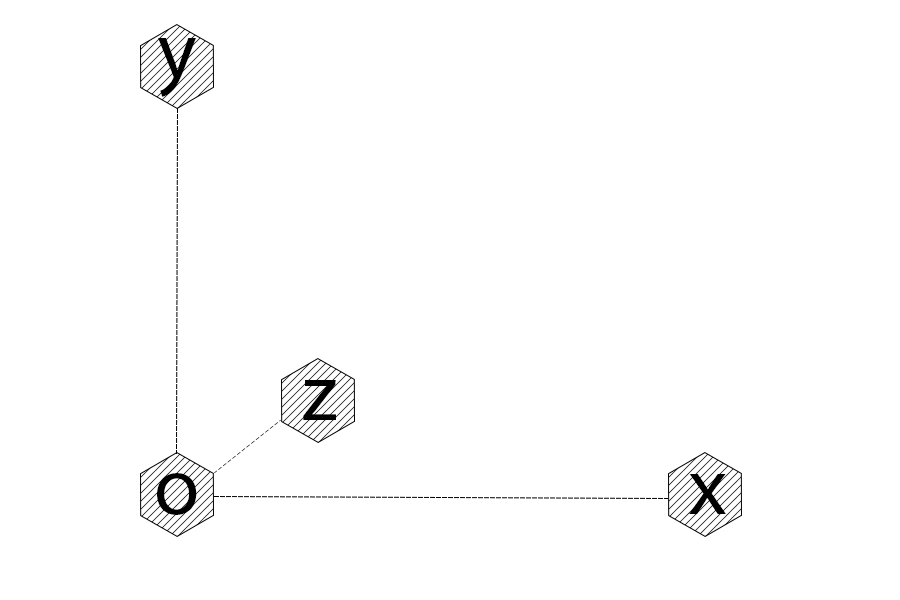
\includegraphics[height=0.2\textheight]{uwb_axis.png}
	\caption{Disposizione ancore}
	\label{fig: disposizione ancore}
\end{figure}
comportamento fisico
tag
anchors, come disporre le ancore \\
autocalibrazione
come gestire flash memory dei device
warning: remote\_id 
problematiche relative al doPositioning veloce (servono le pause)
pacchetto ros custom descrivere in breve cosa fanno i file dentro charlie\_pozyx

%%%%%%%%%%%%%%%%%%%%%%%%%%%%%%%%%%%%%%%%%%%%%%%%%%%%%%%%%%%%%%%%%%%%%%%%%%%%%%%%%%%%%%%%%%%%%%%%%%%%%%
\section{Sistema Vicon}
\label{sez:Sistema Vicon}
come si installa \\
come si crea un oggetto\\
come si calibra

%%%%%%%%%%%%%%%%%%%%%%%%%%%%%%%%%%%%%%%%%%%%%%%%%%%%%%%%%%%%%%%%%%%%%%%%%%%%%%%%%%%%%%%%%%%%%%%%%%%%%%
\section{L'esperimento}
\label{sez:L'esperimento}
procedura con i comandi, ogni cosa che facciamo \`e commentata e descritta \\
albero nodi\\
albero tf\\

%%%%%%%%%%%%%%%%%%%%%%%%%%%%%%%%%%%%%%%%%%%%%%%%%%%%%%%%%%%%%%%%%%%%%%%%%%%%%%%%%%%%%%%%%%%%%%%%%%%%%%
\section{Prove?}
\subsection{Confronto Vicon}

\subsection{Esperimento nel cortile}

\subsection{Esperimento all'aperto}



%%%%%%%%%%%%%%%%%%%%%%%%%%%%%%%%%%%%%%%%%%%%%%%%%%%%%%%%%%%%%%%%%%%%%%%%%%%%%%%%%%%%%%%%%%%%%%%%%%%%%%
\newpage
\section{Guida breve all'esperimento}
In questa sezione \`e scritta, in modo molto sintetico, la procedura per lanciare un esperimento. Per una guida dettagliata rifarsi a sez.~\ref{sez:L'esperimento}. 

Prima di tutto \`e necessario disporre le ancore come descritto in sez.~\ref{sez:Sistema Pozyx} e come si pu\`o vedere in fig.~\ref{fig: disposizione ancore}. Assicurarsi di aver impostato correttamente le impostazioni WiFi (sez.~\ref{sez: primo collegamento a raspberry}) e di avere connessi alla stessa rete pc e Raspberry.


Connettersi \textbf{ssh} con password \texttt{robot}:
\begin{lstlisting}[style=bash]
	ssh -X -C pi@raspberrypi.local		# avvia ssh
\end{lstlisting}

Per l'\textbf{autocalibrazione} (necessaria ogni volta che viene riposizionato il sistema di ancore) lanciare \textbf{ABBIAMO FATTO IL FILE .SH DA CAMBIARE}:
\begin{lstlisting}[style=bash]
	python3 /charlie_autocalibration/autocalibration_ransac.py
\end{lstlisting}
infine rispondere ``y'' per salvare i risultati nella memoria flash delle ancore.

Adesso \`e necessario avviare il \textbf{posizionamento} delle tag pozyx e la comunicazione \textbf{seriale} con Icaro (suggeriamo di utilizzare pi\`u terminali con \href{https://terminator-gtk3.readthedocs.io/en/latest/}{terminator}):
\begin{lstlisting}[style=bash]
	roslaunch charlie_launch start_uwb.launch		# avvia uwb
	roslaunch charlie_launch start_serial.launch	# avvia seriale con stm
\end{lstlisting}

\subsection*{Nuova Mappa}
Una nuova mappa \`e necessaria quando si cambia posizionamento alle ancore o banalmente si cambia luogo. Consigliamo di muovere Charlie attraverso il radiocomando in questa fase.
\begin{lstlisting}[style=bash]
	roslaunch charlie_launch save_map_origin.launch		# con Charlie fermo!
	roslaunch charlie_launch new_map.launch 	# muovere Charlie lentamente
\end{lstlisting}

Una volta soddisfatti del risultato salvare la mappa attraverso:
\begin{lstlisting}[style=bash]
	cd charlie_ws/maps
	rosrun map_server map_saver -f NOME_MAPPA
\end{lstlisting}

\subsection*{Localizzazione}
Sostituire il nome della mappa che si vuole utilizzare nel file

\verb|/home/pi/charlie_ws/src/charlie_launch/launch/localization.launch|:

\huge \textbf{VERIFICARE} \normalsize 
\begin{lstlisting}[style=xml, firstnumber=11]
	<node name="map_server" pkg="map_server" type="map_server" args="/home/pi/charlie_ws/maps/NOME_MAPPA.yaml"/>
\end{lstlisting}

Quindi lanciare:
\begin{lstlisting}[style=bash]
	roslaunch charlie_launch localization.launch
\end{lstlisting}

Nello stesso file \`e possibile impostare di visualizzare rviz attraverso il ``Compressed X11 Forwarding '' scommentando la riga corrispondente di rviz. Questa opzione \`e molto sconsigliata da noi in quanto rende la visione poco reattiva. Per ovviare a questo problema, dopo aver configurato pc e raspberry come descritto in sez.~\ref{sez: Ros master/slave}, \`e possibile lanciare da pc:

\begin{lstlisting}[style=bashPC]
	roslaunch charlie_remote rviz_remote.launch
\end{lstlisting}
In questo momento l'esperimento \`e iniziato!

\subsection*{Waypoints}
\`E possibile indicare una posa-goal tramite il comando \texttt{2DNavgoal} direttamente da rviz (tenere premuto per assegnare l'orientazione).
Per attivare i motori e permettere al robot di spostarsi, pubblicare il seguente messaggio sul topic \verb|start\_and\_stop|:

\begin{lstlisting}[style=bash]
	rostopic pub /start_and_stop std_msgs/Float64 "data: 1.0"
\end{lstlisting}

e per fermarli:

\begin{lstlisting}[style=bash]
	rostopic pub /start_and_stop std_msgs/Float64 "data: 0.0"
\end{lstlisting}

\subsection*{Sistema Vicon}
Ovviamente per utilizzare il sistema Vicon \`e necessario essere nella stanza del volo. Per l'installazione rifarsi a sez.~\ref{sez:Sistema Vicon}. Una volta che il sistema \`e in funzione, avviare l'applicazione di tracking \textbf{SCRIVERE NOME PER BENE} e selezionare nella lista oggetti: \texttt{Charlie} e \texttt{WAND NOME PER BENE}.

Per avviare i dialoghi tra ros e il sistema Vicon avviare da pc:
\begin{lstlisting}[style=bashPC]
	roslaunch charlie_remote vicon_charlie.launch
\end{lstlisting}

poi salvare la trasformazione tra vicon e uwb (richiede il posizionamento della wand sulle ancore):
\begin{lstlisting}[style=bashPC]
	rosrun charlie_remote vicon2uwb_tf.py
\end{lstlisting}

e infine lanciare il nodo che pubblica la posizione di Charlie in frame map:
\begin{lstlisting}[style=bashPC]
	rosrun charlie_remote charlie_vicon2map.py
\end{lstlisting}


\subsection*{Rosbag}
Per registrare i dati attraverso una rosbag suggeriamo di non sottroiscriversi a tutti i topic ma quindi di lanciare il seguente comando da pc (dopo essersi spostati nella cartella desiderata):
\begin{lstlisting}[style=bashPC]
	rosbag record /clock /initialpose /map /orientation /particlecloud /robot_pose /rosout /rosout_agg /scan /tag_center /tf /amcl_pose /charlie_vicon_map -O NOME_BAG.bag
\end{lstlisting}

Per eseguire i topic necessari a AMCL, prima riconfigurare il file:

\verb|../charlie_remote/launch/exec_bash.launch| con i file e il path che si vogliono utilizzare e quindi lanciare da pc:
\begin{lstlisting}[style=bashPC]
	roslaunch charlie_remote exec_bag.launch
\end{lstlisting}
e da raspberry:
\begin{lstlisting}[style=bash]
	roslaunch charlie_launch localization_bag.launch
\end{lstlisting}

%%%%%%%%%%%%%%%%%%%%%%%%%%%%%%%%%%%%%%%%%%%%%%%%%%%%%%%%%%%%%%%%%%%%%%%%%%
\newpage
\appendix
\section{Autocalibrazione}
L'autocalibrazione si basa sullo script \texttt{python3} ``autocalibration\_ransac.py''. 
Per farlo funzionare occorre per prima cosa avere quattro ancore correttamente alimentate ed un dispositivo Pozyx connesso, il quale servirà da comunicazione seriale tra la rete Pozyx e l’utente. 
Il dispositivo seriale può, a discrezione dell’utente, essere un’ancora o un tag. 
É possibile, se si desidera, effettuare una calibrazione manuale delle ancore, andando a settare la variabile \verb|autoCal| a \verb|True|. 
In tal caso si dovrà utilizzare un metro per misurare la distanza relativa tra le coppie di ancore della rete ed inserire manualmente i valori misurati nelle opportune variabili \texttt{r01}, \texttt{r02}, \texttt{r03}, \texttt{r12}, \texttt{r13} ed \texttt{r23}, che rappresentano le distanze tra le rispettive antenne.
Per quanto riguarda invece la calibrazione automatica, lo script prevede una fase di acquisizione dei dati necessari, successivamente viene eseguito l’algoritmo ransac ed infine viene utilizzato l’algoritmo algebrico per determinare le coordinate effettive delle ancore. 
L’algoritmo ransac rimuove eventuali outliers dalle misurazioni delle distanze relative tra le antenne e fornisce quindi una stima della distanza tra ciascuna coppia di ancore basata sui dati senza outliers.
Nel corso della procedura di autocalibrazione vengono stampati sul terminale vari dati, tra cui i fondamentali sono:
\begin{itemize}
	\item Coordinate dei dispositivi all’accensione del sistema, prima che sia effettuata la nuova calibrazione;
	
	\item Risultato del settaggio dei parametri UWB della rete;
	
	\item Il risultato dell’algoritmo ransac per la distanza tra le ancore;
	
	\item Risultato dell'algoritmo algebrico per determinare le coordinate delle ancore: se tale algoritmo fallisca, \`e mostrato su terminale l'errore;
\end{itemize}



% Bibliography
\newpage
\bibliography{biblio}


\end{document}